%%%%%%%%%%%%%%%%%%%%%%%%%%%%%%%%%%%%%%%%%
% Beamer Presentation
% LaTeX Template
% Version 1.0 (10/11/12)
%
% This template has been downloaded from:
% http://www.LaTeXTemplates.com
%
% License:
% CC BY-NC-SA 3.0 (http://creativecommons.org/licenses/by-nc-sa/3.0/)
%
%%%%%%%%%%%%%%%%%%%%%%%%%%%%%%%%%%%%%%%%%

%----------------------------------------------------------------------------------------
%	PACKAGES AND THEMES
%----------------------------------------------------------------------------------------

\documentclass{beamer}

\mode<presentation> {

% The Beamer class comes with a number of default slide themes
% which change the colors and layouts of slides. Below this is a list
% of all the themes, uncomment each in turn to see what they look like.

%\usetheme{default}
%\usetheme{AnnArbor}
%\usetheme{Antibes}
%\usetheme{Bergen}
%\usetheme{Berkeley}
%\usetheme{Berlin}
%\usetheme{Boadilla}
%\usetheme{CambridgeUS}
%\usetheme{Copenhagen}
%\usetheme{Darmstadt}
%\usetheme{Dresden}
%\usetheme{Frankfurt}
%\usetheme{Goettingen}
%\usetheme{Hannover}
%\usetheme{Ilmenau}
%\usetheme{JuanLesPins}
%\usetheme{Luebeck}
\usetheme{Madrid}
%\usetheme{Malmoe}
%\usetheme{Marburg}
%\usetheme{Montpellier}
%\usetheme{PaloAlto}
%\usetheme{Pittsburgh}
%\usetheme{Rochester}
%\usetheme{Singapore}
%\usetheme{Szeged}
%\usetheme{Warsaw}

% As well as themes, the Beamer class has a number of color themes
% for any slide theme. Uncomment each of these in turn to see how it
% changes the colors of your current slide theme.

%\usecolortheme{albatross}
%\usecolortheme{beaver}
%\usecolortheme{beetle}
%\usecolortheme{crane}
%\usecolortheme{dolphin}
%\usecolortheme{dove}
%\usecolortheme{fly}
%\usecolortheme{lily}
%\usecolortheme{orchid}
%\usecolortheme{rose}
%\usecolortheme{seagull}
%\usecolortheme{seahorse}
%\usecolortheme{whale}
%\usecolortheme{wolverine}

%\setbeamertemplate{footline} % To remove the footer line in all slides uncomment this line
%\setbeamertemplate{footline}[page number] % To replace the footer line in all slides with a simple slide count uncomment this line

%\setbeamertemplate{navigation symbols}{} % To remove the navigation symbols from the bottom of all slides uncomment this line
}

\usepackage{graphicx} % Allows including images
\usepackage{booktabs} % Allows the use of \toprule, \midrule and \bottomrule in tables
\usepackage{listings}
\usepackage{caption}
\usepackage{subcaption}
\captionsetup{compatibility=false}
\usepackage[backend=bibtex, style=authoryear]{biblatex}
\addbibresource{mybib.bib}

\graphicspath{ {../plots/} }

\hypersetup{
	colorlinks=true,
	linkcolor=red,
	filecolor=magenta,
	urlcolor=blue,
}

\newenvironment{graytext}{\color{gray}}{\ignorespacesafterend}

%----------------------------------------------------------------------------------------
%	TITLE PAGE
%----------------------------------------------------------------------------------------

\title[Cornell CS5356 Fall 2015]{Analytics} % The short title appears at the bottom of every slide, the full title is only on the title page

\author{Ilya Kavalerov} % Your name
\institute[UMD] % Your institution as it will appear on the bottom of every slide, may be shorthand to save space
{
University of Maryland \\ % Your institution for the title page
Electrical and Computer Engineering \\
\medskip
\textit{ilyak@umiacs.umd.edu} % Your email address
}
\date{\today} % Date, can be changed to a custom date

\begin{document}

\begin{frame}
\titlepage % Print the title page as the first slide
\end{frame}

%------------------------------------------------

\begin{frame}
	\frametitle{About me}
	\begin{itemize}
		\item Previously at Artsy (backend engineer, prediction)
		\item PhD Student at EECE department at UMD, Signal Processing
	\end{itemize}
	
	\begin{figure}
		\centering
		\begin{subfigure}{.5\textwidth}
			\centering
			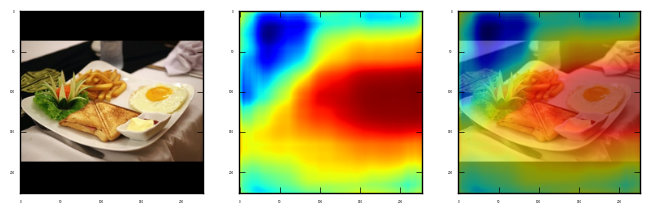
\includegraphics[width=1\linewidth]{3897517_class28_overlaid_heatmap}
		\end{subfigure}%
		\begin{subfigure}{.5\textwidth}
			\centering
			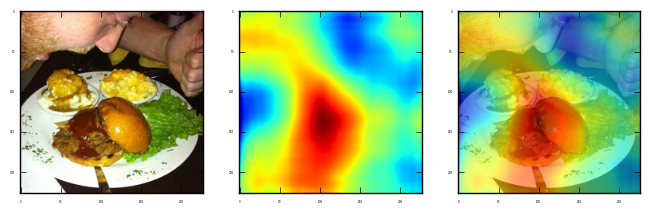
\includegraphics[width=1\linewidth]{925105_class80_overlaid_heatmap}
		\end{subfigure}
		\caption{Egg and Burger detection}
	\end{figure}
	
\end{frame}

%------------------------------------------------

\begin{frame}
	\frametitle{Overview}
	\begin{itemize}
		\item Why be data driven?
		\item New kinds of problems introduced by learning
		\item Some simple examples of using typical business data
	\end{itemize}
\end{frame}

%------------------------------------------------

\begin{frame}
	\frametitle{Data at work}
	\begin{itemize}
		\item Data driven/Data-curious culture (SQL and graph friendly)
		\item Kaizen
		\item Why the "big data" hype?
			\begin{itemize}
				\item Magic bullet image
				\item abundance of fuel (\textbf{heuristics} become harder, \textbf{learning} becomes more effective) eg. Face recognition, 30TB = 1yr Duke heart center, 1 day Fb, 1 s CERN
			\end{itemize}		
			\begin{figure}
				\centering
				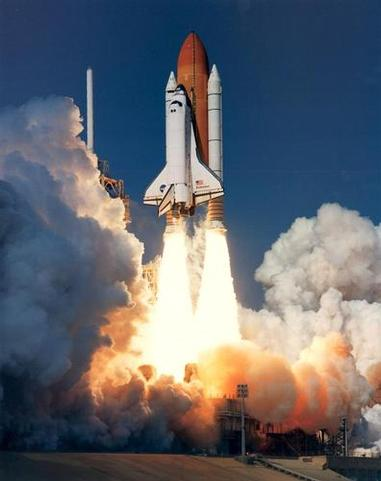
\includegraphics[width=0.25\linewidth]{rocket}
			\end{figure}
			\item Extract new forms of value from information
	\end{itemize}
\end{frame}

%------------------------------------------------

\begin{frame}
	\frametitle{How others use data: The job}
	\begin{itemize}
		\item "Data scientist"
		\begin{itemize}
			\item 2008 from LinkedIn Job posting by DJ Patil and Jeff Hammerbacher
			\item 2012 Wikipedia Entry, HBR's \href{https://hbr.org/2012/10/data-scientist-the-sexiest-job-of-the-21st-century/}{Sexiest job of 21st century}
			\item Statistics, Data munging, Visualization
		\end{itemize}
	\end{itemize}
	\begin{figure}
		\centering
		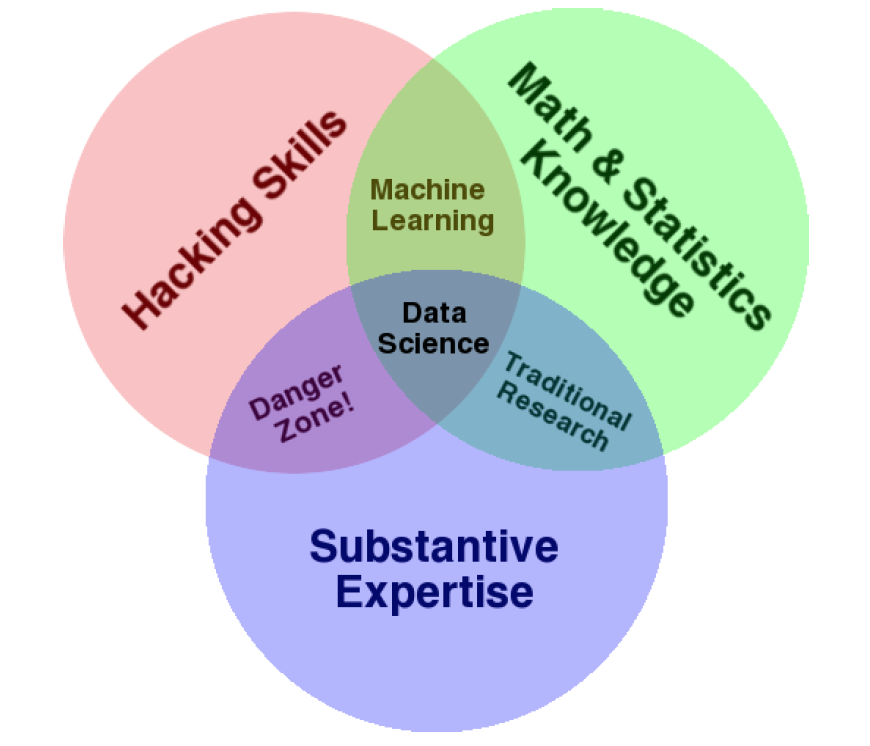
\includegraphics[width=0.4\linewidth]{drew_conway}
		\caption{Drew Conway's diagram}
	\end{figure}
\end{frame}

%------------------------------------------------

\begin{frame}
	\frametitle{How others use data: Learn a model}
	\begin{itemize}
		\item Maximum Likelihood: Maximize probability of your data given a model
		\item iid assumption: $p(x_1,x_2, \cdots , x_n | \Theta) = p(x_1|\Theta)\times p(x_2|\Theta) \times \cdots \times p(x_n|\Theta)$
	\end{itemize}
	$$\Theta^* = \mathrm{argmax}_\Theta  \prod_{i=1}^N p(x_i | \Theta) = \mathrm{argmax}_\Theta  \sum_{i=1}^N \log p(x_i | \Theta) $$
	\begin{figure}
		\centering
		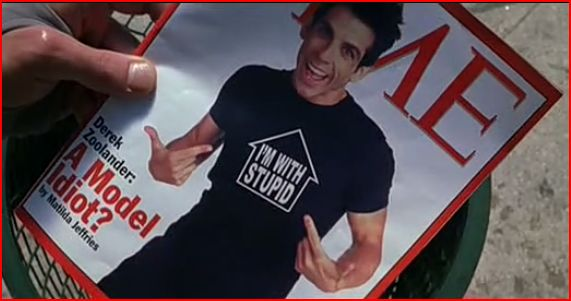
\includegraphics[width=0.5\linewidth]{model_idiot}
	\end{figure}
\end{frame}

% page 11 last
%------------------------------------------------

\begin{frame}
	\frametitle{Dangers: Machine learning disrupts software engineering}
	
	\begin{columns}
		\column{0.7\linewidth}
		\centering
		\begin{itemize}
			\item Abstraction = leverage works of others
			\item Engineer complex artifacts (Airplane: 3M parts, Debian: 0.4B LOC)
			\item We expect to use programs much like we use math theorems (design contracts)
			\item Abstraction leaks limit complexity (Snowplow)
			\begin{itemize}
				\item Sorting has few assumptions on input (only obvious failure is performance)
				\item Using a learned model has huge assumptions on input (understanding these is the hard part)
			\end{itemize}
		\end{itemize}
		\column{0.3\linewidth}
		\centering
		\begin{figure}
			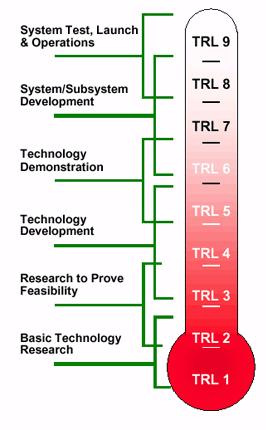
\includegraphics[width=1\linewidth]{NASA_TRL_Meter}
			\caption{\href{https://en.wikipedia.org/wiki/Technology_readiness_level}{NASA Technology Readiness Levels}}
		\end{figure}
	\end{columns} 
\end{frame}

%------------------------------------------------

\begin{frame}
	\frametitle{In short: Don't go overboard}
	\begin{itemize}
		\item "Great products are a convergence of the right set of technologies" - Jon Rubinstein (EE behind the first iPod)
		\item Do simple things with few assumptions for less surprises
		\item Track everything, ask questions later
	\end{itemize}
	\begin{figure}
		\centering
		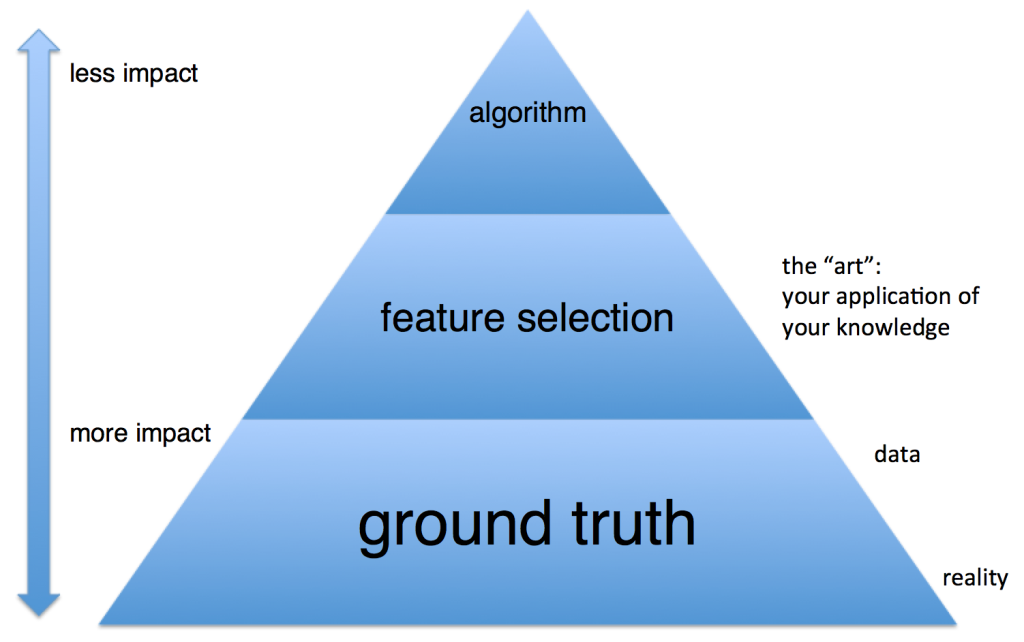
\includegraphics[width=0.4\linewidth]{alex_pinto}
		\caption{Chart inspired by a slide from Alex Pinto's talk,  \href{https://www.youtube.com/watch?v=TYVCVzEJhhQ}{"Secure Because Math: A Deep-Dive on ML-Based Monitoring"}}
	\end{figure}
	\begin{itemize}
		\item Iterative/Continuous improvements in the startup spirit
	\end{itemize}
\end{frame}

%------------------------------------------------

\begin{frame}
	\frametitle{Conditional Probability \& Baye's rule}
	\begin{itemize}
		\item $p(X|Y) = \frac{p(X,Y)}{p(Y)}$
		\item $p(\Theta|X) = \frac{p(X|\Theta)p(\Theta)}{p(X)}$
		\item posterior = $\frac{\mathrm{likelihood} \times \mathrm{prior} }{\mathrm{evidence}}$
		\item We'll use this in the following example: Subscription tiers on BriskIT, Free, \$Monthly, and \$\$Yearly. Say we want to run a promotion on the yearly subscription, we decide to A/B Test 2 methods to convert users
	\end{itemize}
\end{frame}

%------------------------------------------------

\begin{frame}
	\frametitle{BriskIT Subtle Banner}
	\begin{figure}
		\centering
		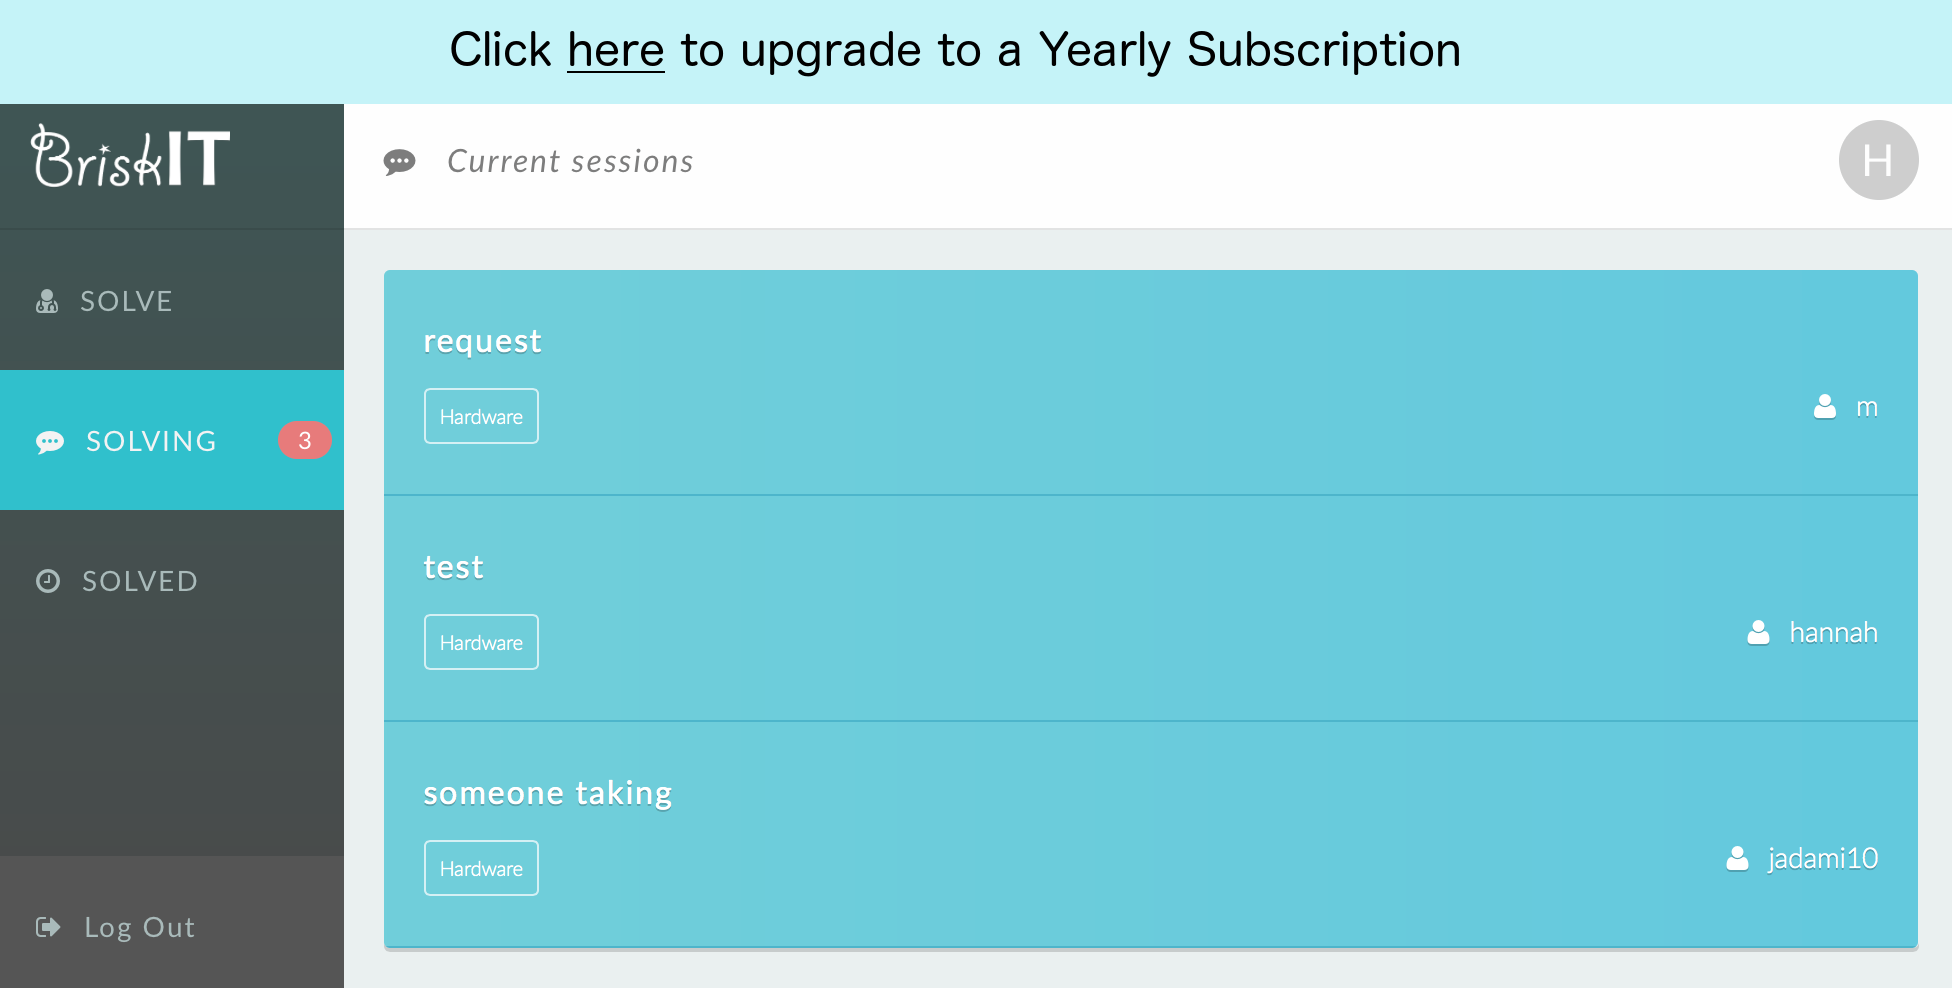
\includegraphics[width=1\linewidth]{briskit_banner}
	\end{figure}
\end{frame}

%------------------------------------------------

\begin{frame}
	\frametitle{BriskIT Pop-up}
	\begin{figure}
		\centering
		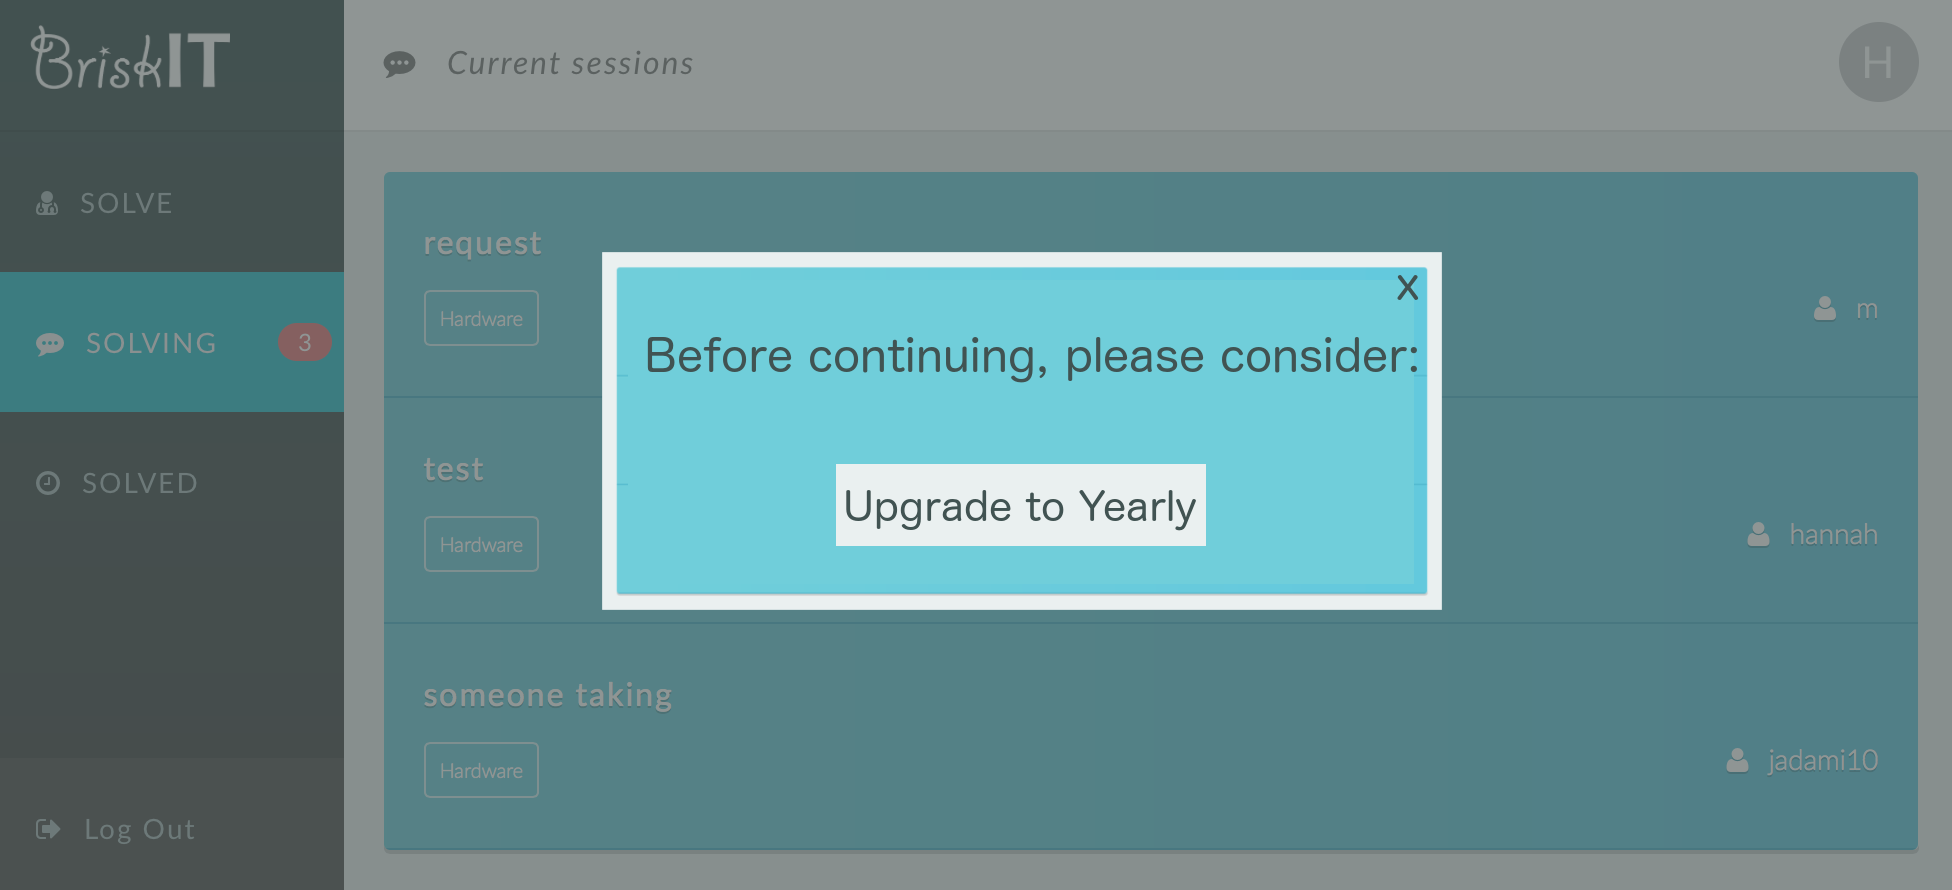
\includegraphics[width=1\linewidth]{briskit_popup}
	\end{figure}
\end{frame}

%------------------------------------------------

\begin{frame}
	\frametitle{Simpson's Paradox: 1}
	\begin{itemize}
		\item Subscription tiers on BriskIT, Free, \$Monthly, and \$\$Yearly. Say we want to run a promotion on the yearly subscription, we get the results of an A/B Test on 2 methods to convert users:
	\end{itemize}
	\begin{table}
		\begin{tabular}{|c|c|c|}
			 & Pop Up & Subtle Banner
			\onslide<1>{\\\hline} Users (Converted/Total) & 78\% (273/350) & 83\% (289/350)
		\end{tabular}
	\end{table}
	\begin{itemize}
		\item Looks like subtle banner wins. But with more features $\dots$
	\end{itemize}
\end{frame}

%------------------------------------------------

\begin{frame}
	\frametitle{Simpson's Paradox: 2}
	\begin{itemize}
		\item With more features:
	\end{itemize}
	\begin{table}
		\begin{tabular}{|c|c|c|}
			& Pop Up & Subtle Banner
			\onslide<1>{\\\hline} Monthly Subscribers & 93\% (81/87) & 87\% (234/270)
			\onslide<1>{\\\hline} Free Users & 73\% (192/263) & 69\% (55/80)
			\onslide<1>{\\\hline} Users (Converted/Total) & 78\% (273/350) & 83\% (289/350)
		\end{tabular} 
	\end{table}
	\begin{itemize}
		\item The less effective method (Subtle Banner) is tested on the easier cases more often $\not \Rightarrow$ Subtle Banner is more effective
	\end{itemize}
\end{frame}

%------------------------------------------------

\begin{frame}
	\frametitle{Simpson's Paradox: 3}
	\begin{itemize}
		\item Okay it's intuitive, our bad pitch (subtle banner) got the easy targets (already subscribers), but let's express this with a probability.
	\end{itemize}
	\begin{table}
		\begin{tabular}{|c|c|c|}
			& Pop Up & Subtle Banner
			\onslide<1>{\\\hline} Monthly Subscribers & 93\% (81/87) & 87\% (234/270)
			\onslide<1>{\\\hline} Free Users & 73\% (192/263) & 69\% (55/80)
			\onslide<1>{\\\hline} Users (Converted/Total) & 78\% (273/350) & 83\% (289/350)
		\end{tabular} 
	\end{table}
	\begin{itemize}
		\item $p( $Monthly$ ) = \frac{87+270}{87+270+263+80} = 0.51$
	\end{itemize}
\end{frame}

%------------------------------------------------

\begin{frame}
	\centerline{Bizsouk: Material sourcing platform for industries}
	\centerline{Visualize last 1000 trades}
	\Huge{\centerline{Demo}}
\end{frame}

%------------------------------------------------

\begin{frame}
	\frametitle{Zipf's Law}
	\begin{itemize}
		\item Total income a function of heaviest hitter's income $A$: $\frac{A}{1} + \frac{A}{2} + \cdots + \frac{A}{n}$
		\item Upward convexity is a condition of surfeit (too few are getting too much, diversification will follow), downward convexity is a condition of deficiency
		\item Long tail, can be similar to log normal
		% similarity to log normal
		% at least get a mean and estimate from that
	\end{itemize}
	\begin{figure}
		\centering
		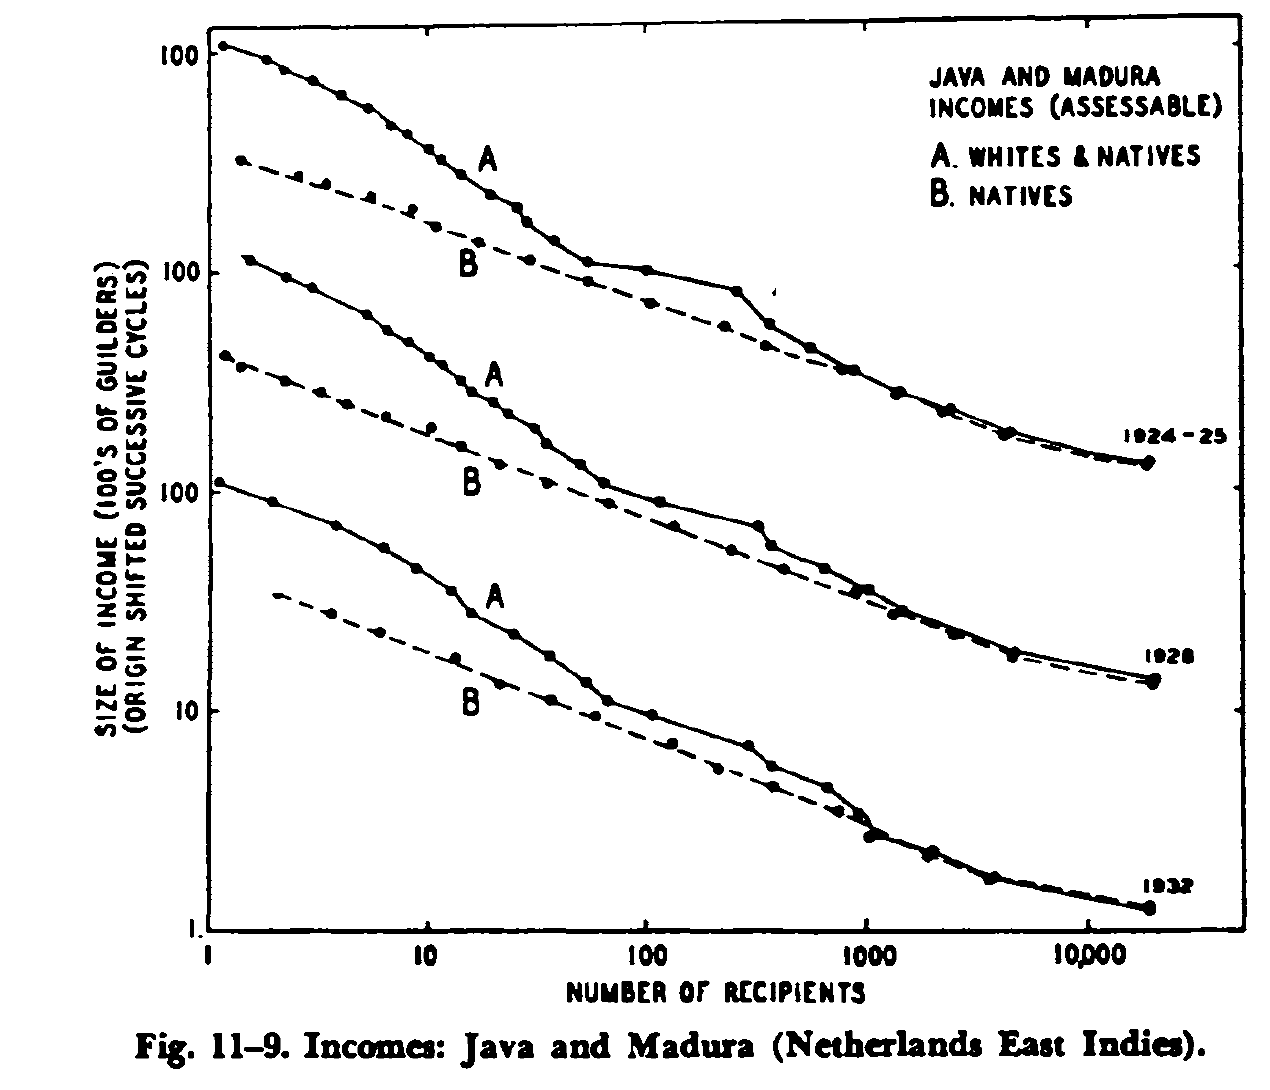
\includegraphics[width=0.4\linewidth]{zipf}
		\caption{From Zipf's Principle of least effort. Power changed hands by 1949.}
	\end{figure}
\end{frame}

%------------------------------------------------

\begin{frame}
	\centerline{Artrank}
	\centerline{Is Frank Stella undervalued according to Artsy Auction Prices?}
	\Huge{\centerline{Demo}}
	\begin{figure}
		\centering
		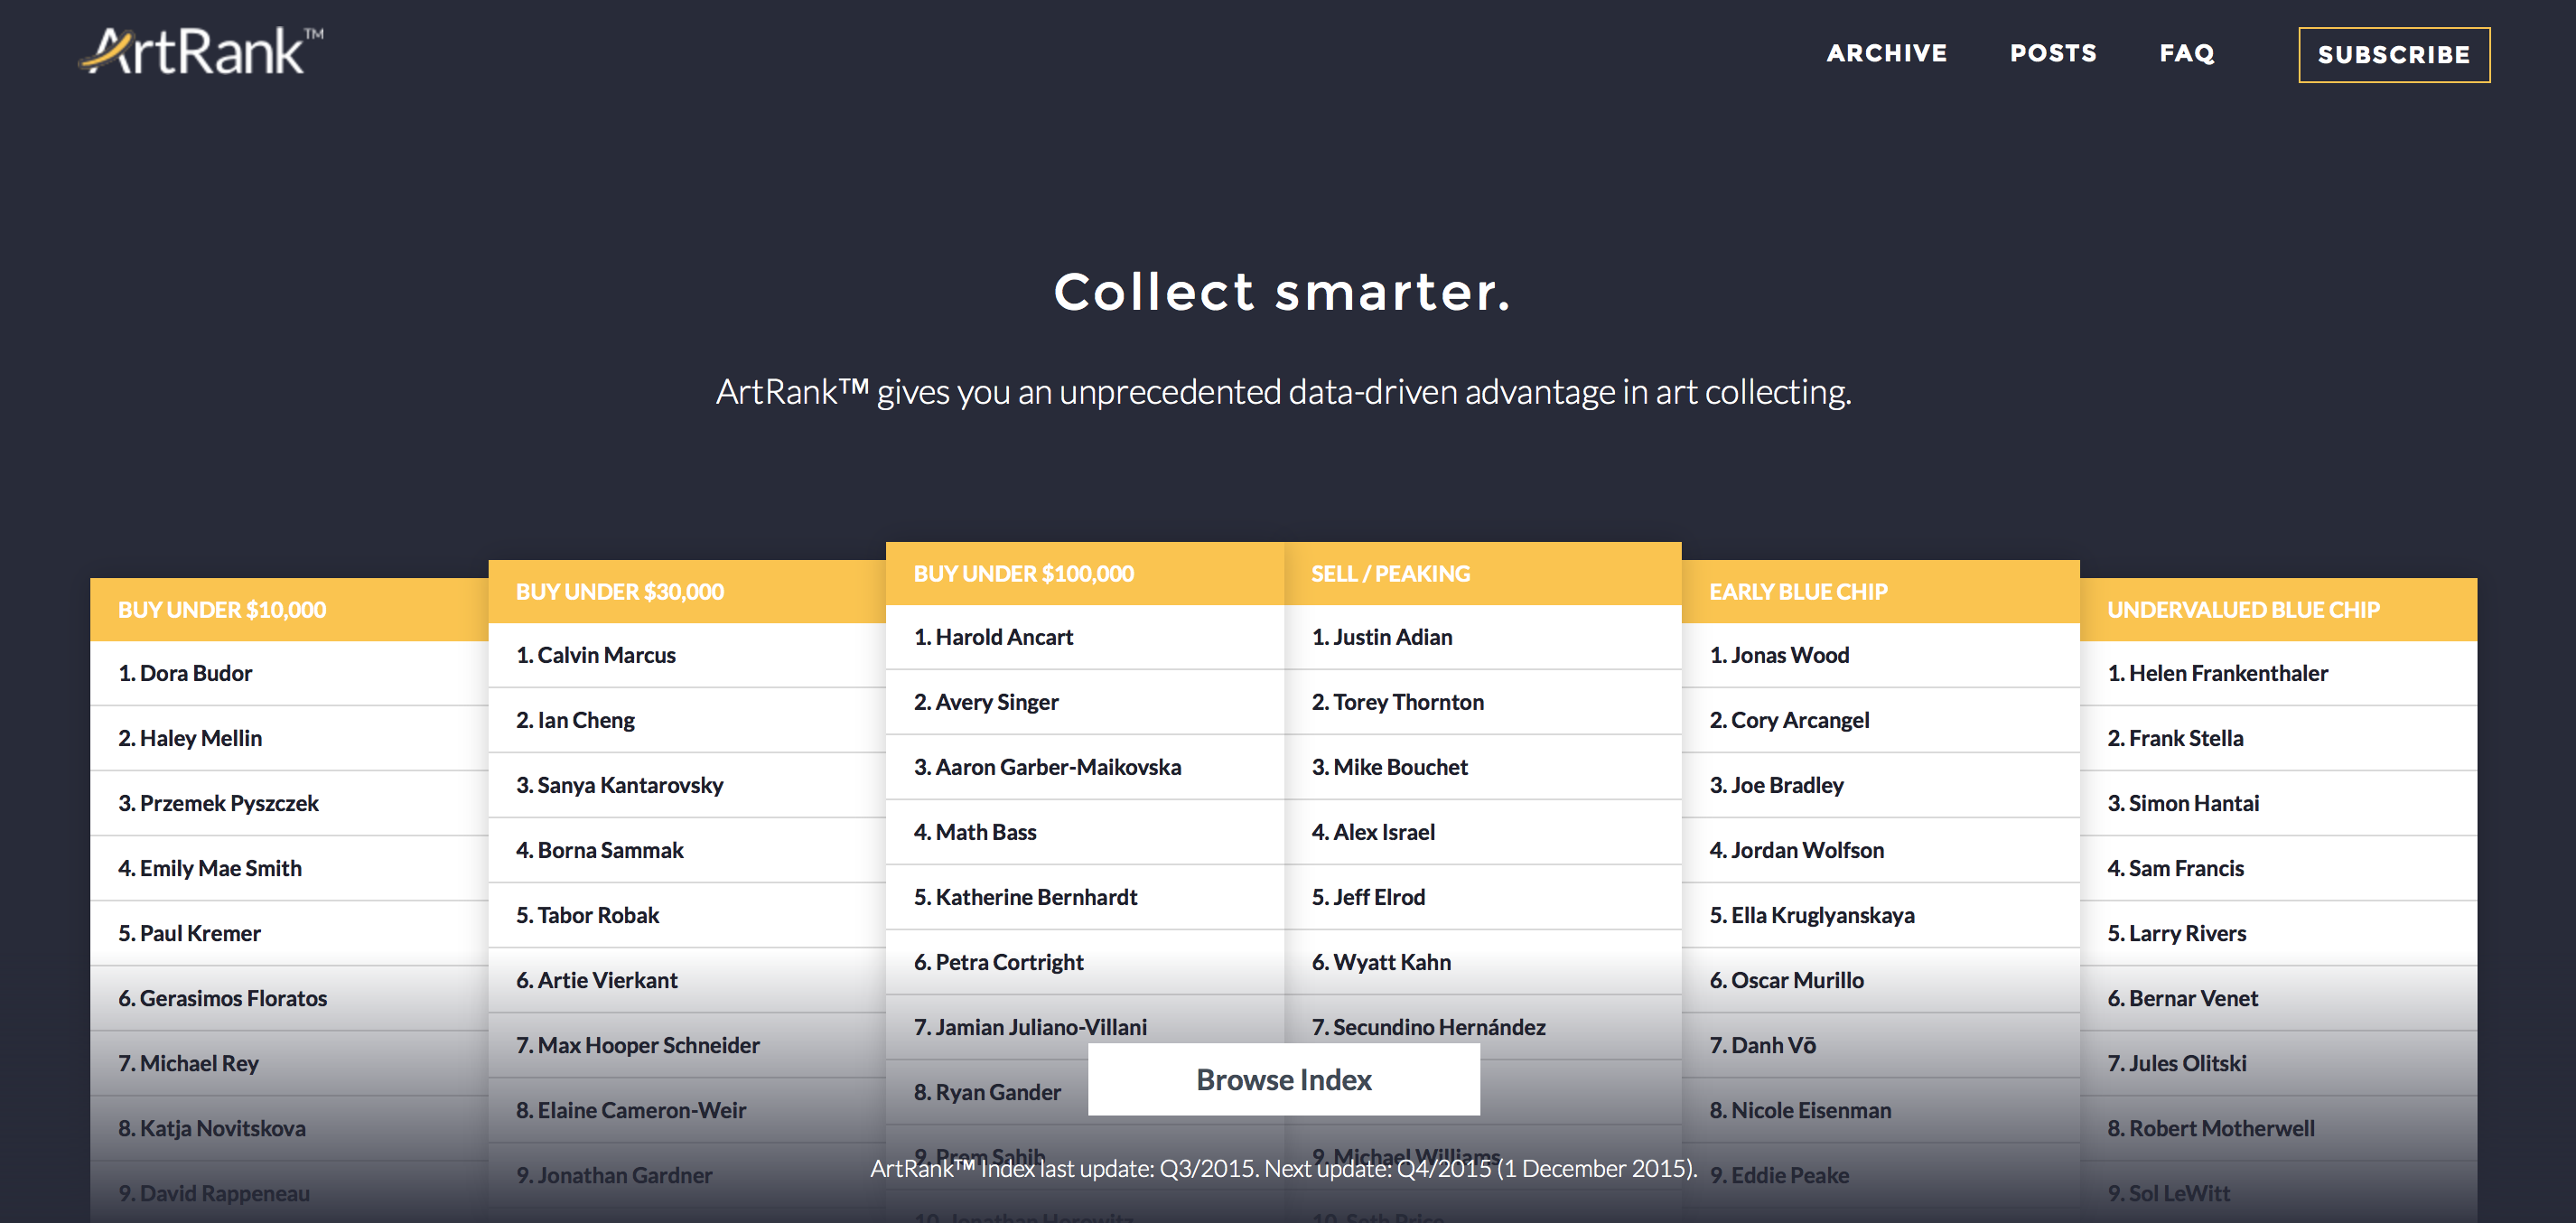
\includegraphics[width=0.8\linewidth]{artrank}
	\end{figure}
\end{frame}

%------------------------------------------------

\begin{frame}
	\centerline{Gitrank: Featured OS Libraries}
	\centerline{Find undervalued game engines}
	\Huge{\centerline{Demo}}
	\begin{figure}
		\centering
		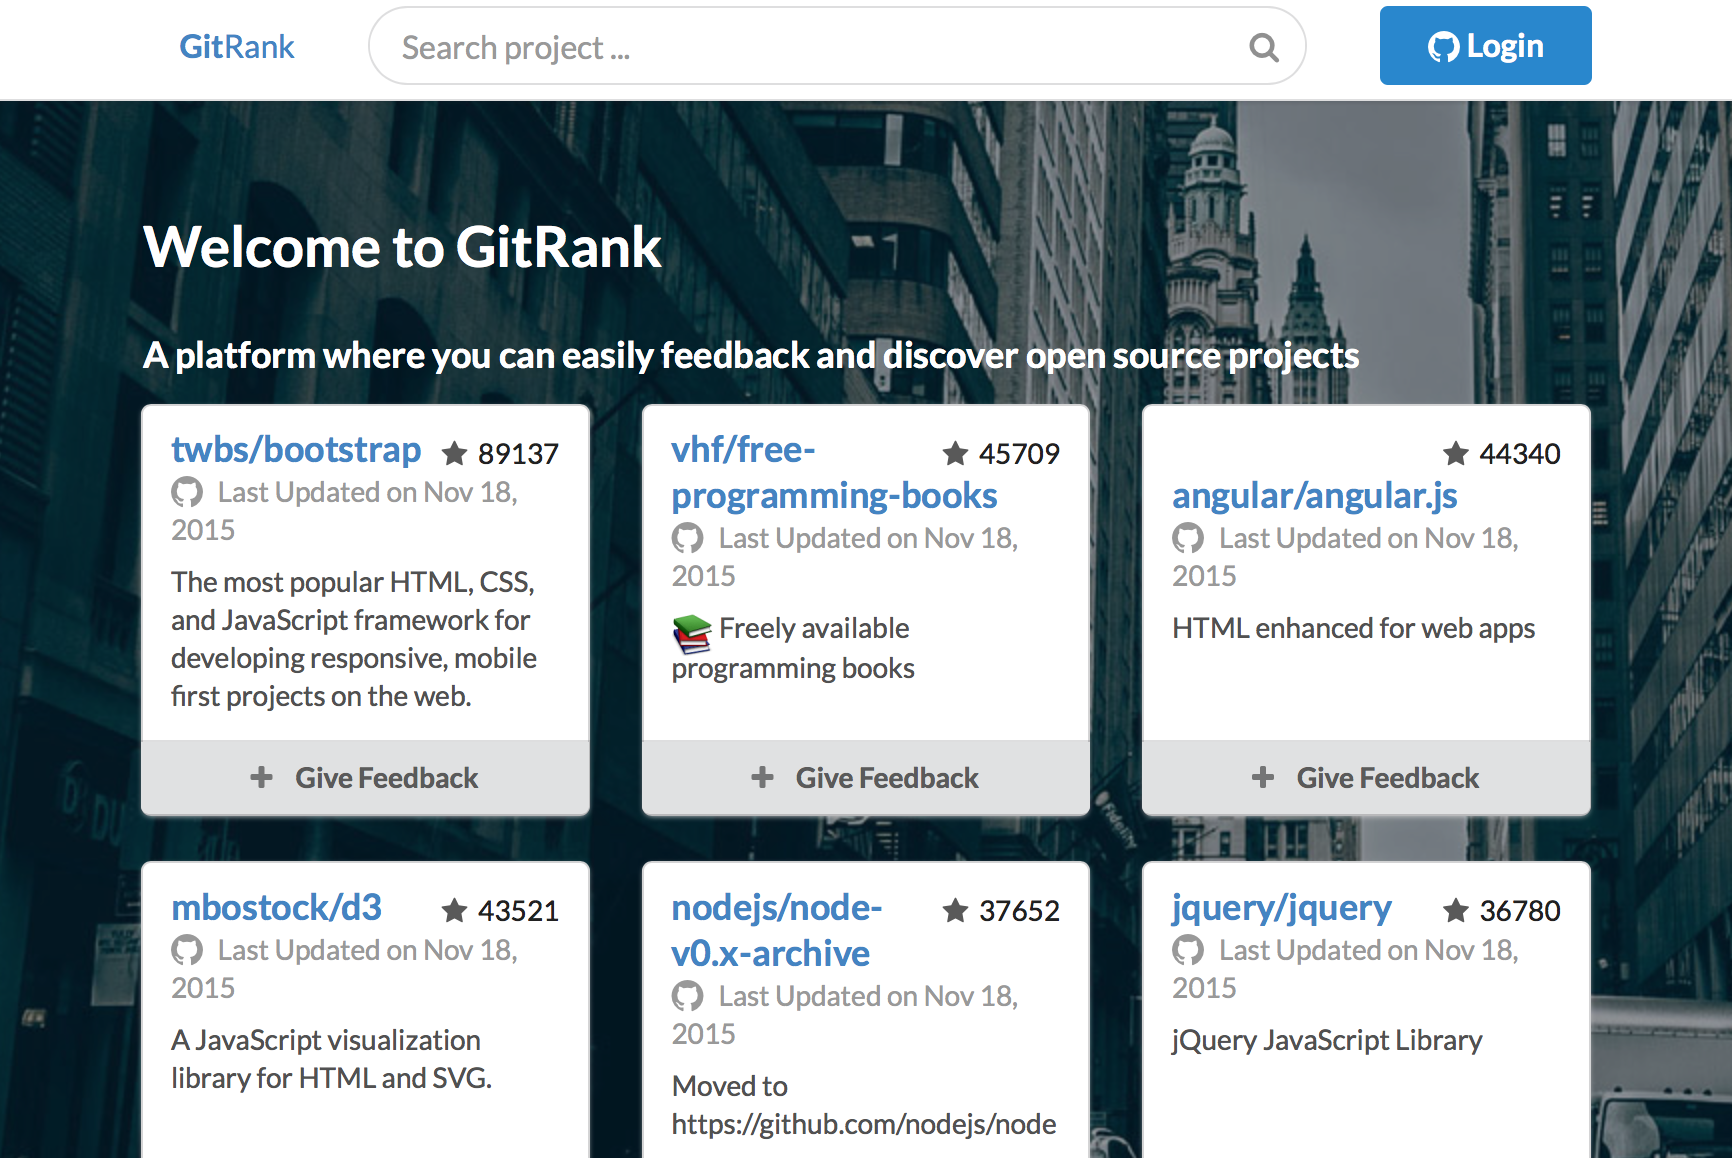
\includegraphics[width=0.8\linewidth]{gitrank}
	\end{figure}
\end{frame}

%------------------------------------------------

\begin{frame}
	\frametitle{Conclusion}
	\begin{itemize}
		\item Data driven decision making can lead to quicker/more continuous improvements
		\item It's easy to fall into doing research, keep it simple
		\item Some examples similar to what I saw while working
	\end{itemize}
\end{frame}

%------------------------------------------------

\begin{frame}
	\Huge{\centerline{Thank You!}}
\end{frame}

%------------------------------------------------

\begin{frame}
	\frametitle{References \& Further reading}
	\begin{itemize}
		\item \href{https://labs.spotify.com/puzzles/}{Spotify Labs puzzles}
		\item \href{https://www.dataquest.io/blog/python-data-visualization-libraries/}{Dataquest visualization}
		\item \href{https://github.com/hangtwenty/dive-into-machine-learning/blob/master/README.md}{Dive into Machine Learning}
		\item \href{http://www.amazon.com/Doing-Data-Science-Straight-Frontline/dp/1449358659}{Doing data science: Straight talk from the frontline}
		\item \href{http://www.amazon.com/Human-Behavior-Principle-Least-Effort/dp/161427312X}{Human Behavior and the Principle of Least Effort: An Introduction to Human Ecology}
	\end{itemize}
\end{frame}

\end{document}